\documentclass[11pt,a4paper]{article}
\usepackage{fontspec}
\setmainfont{STIXTwoText-Regular.otf}[BoldFont=STIXTwoText-Bold.otf,ItalicFont=STIXTwoText-Italic.otf,BoldItalicFont=STIXTwoText-BoldItalic.otf]
\setsansfont{texgyreheros-regular.otf}
\setmonofont{texgyrecursor-regular.otf}[Scale=0.82]
\usepackage[margin=24mm,headheight=15pt]{geometry}
\usepackage{amsmath,amssymb,amsthm,mathtools,bm,mathrsfs,microtype}
\newtheorem{proposition}{Proposition}[section]
\newcommand{\dd}{\,\mathrm d}
\newcommand{\R}{\mathbb R}
\newcommand{\C}{\mathbb C}
\DeclareMathOperator{\Rea}{Re}
\DeclareMathOperator{\Ima}{Im}
\usepackage{booktabs,longtable,array,calc,graphicx,xcolor}
\usepackage{caption}
\newcounter{none}
\usepackage{fancyvrb,framed,upquote}
\usepackage{tikz}
\usetikzlibrary{arrows.meta,positioning}
\usepackage[backend=biber,style=numeric,sorting=none,doi=true,url=false,isbn=false]{biblatex}
\addbibresource{../references.bib}
\usepackage[colorlinks=true,linkcolor=blue!45!black,urlcolor=blue!50!black,citecolor=blue!45!black]{hyperref}
\usepackage{bookmark,fancyhdr}
\pagestyle{fancy}
\fancyhf{}
\fancyhead[L]{\small Acoustic Freeform Lab}
\fancyhead[R]{\small SSL generator: vision and theory}
\fancyfoot[C]{\thepage}
\setlength{\parindent}{0pt}
\setlength{\parskip}{0.45em}
\setlength{\emergencystretch}{3em}
\providecommand{\tightlist}{\setlength{\itemsep}{0pt}\setlength{\parskip}{0pt}}
\providecommand{\pandocbounded}[1]{#1}
\numberwithin{equation}{section}
\hypersetup{pdftitle={Programmable stigmatic singlet lenses: vision and theoretical framework},pdfauthor={Acoustic Freeform Lab}}
\title{Programmable stigmatic singlet lenses\\[0.6em]
\large A fixed-prescription acoustic compiler\\Vision, theoretical framework, and verification contract}
\author{Acoustic Freeform Lab\\\small Private research design report}
\date{24 September 2026 --- Version 1.2: multi-fluid variational foundation}
\begin{document}
\maketitle
\begin{abstract}
We start from a vessel containing multiple immiscible fluids and a prescribed
collection of admissible three-dimensional interfaces. A constrained shape
Lagrangian identifies the required mechanical traction as the multiplier of
the desired geometry, with pressure gauge freedom determined by compartment
volumes and connectivity. A viscous Rayleighian extends this inverse to
compatible interface velocities; an inertial weak formulation states its
limits. Only after establishing this load problem do we introduce continuous
acoustic sources, finite-array amplitude and phase optimization, and coupled
forward verification. Cartesian singlets are a later target specialization
with user-supplied conjugates, thickness and frame radius. Stationary accuracy,
stability, formation and adaptive transitions are distinct claims. This is a
mathematical design specification, not a universal realizability theorem or
an experimental validation.
\end{abstract}
\begin{center}
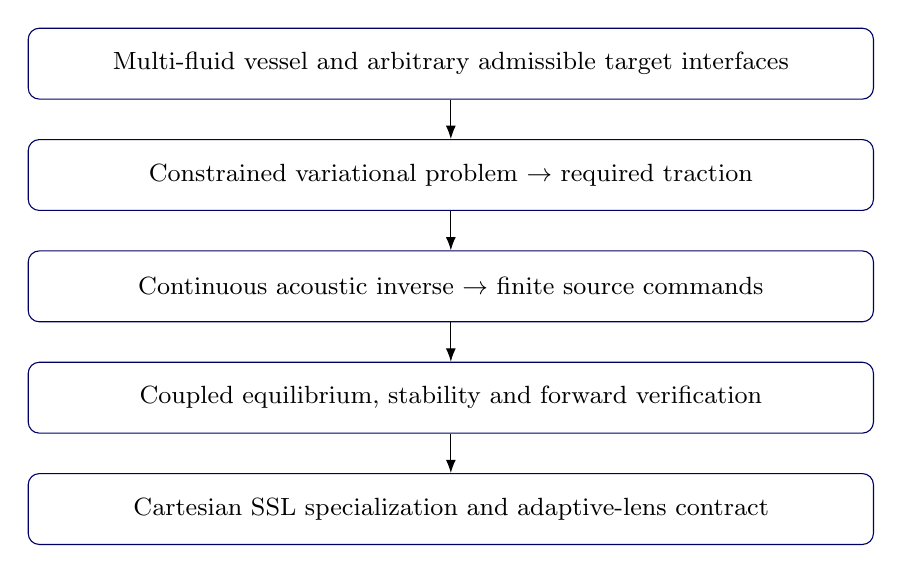
\begin{tikzpicture}[node distance=5mm,box/.style={draw=blue!40!black,rounded corners,align=center,text width=105mm,minimum height=9mm,font=\small},>=Latex]
\node[box] (a) {Multi-fluid vessel and arbitrary admissible target interfaces};
\node[box,below=of a] (b) {Constrained variational problem $\rightarrow$ required traction};
\node[box,below=of b] (c) {Continuous acoustic inverse $\rightarrow$ finite source commands};
\node[box,below=of c] (d) {Coupled equilibrium, stability and forward verification};
\node[box,below=of d] (e) {Cartesian SSL specialization and adaptive-lens contract};
\draw[->] (a)--(b); \draw[->] (b)--(c); \draw[->] (c)--(d); \draw[->] (d)--(e);
\end{tikzpicture}
\end{center}
\clearpage
\tableofcontents
\clearpage
\part{Mathematical formulation and derivations}
\section{The multi-fluid problem for a prescribed shape}
\label{sec:multifluid-start}
The starting point is a desired collection of fluid interfaces, not an
optical prescription or an emitter array. The two questions are:
\emph{which mechanical tractions support the prescribed shape, and which
admissible sources can realize those tractions?} Cartesian lenses are a
later specialization of the target geometry.

\subsection{Domains, interfaces and admissible data}
A fixed bounded vessel $\mathcal D\subset\R^3$ contains $L$ connected fluid
regions $\Omega_\ell(\Gamma)$ separated by $J$ smooth interfaces
$\Gamma=(\Gamma_1,\ldots,\Gamma_J)$. On each interface choose a normal
$\mathbf n_j$ from region $\ell_j^-$ to region $\ell_j^+$. Define
\begin{equation}\label{eq:mf-conventions}
 [\rho]_j^- =\rho_{\ell_j^-}-\rho_{\ell_j^+},\qquad
 [T]_j=T_{\ell_j^+}-T_{\ell_j^-},\qquad
 \kappa_j=\nabla_{\Gamma_j}\cdot\mathbf n_j.
\end{equation}
Thus an outward normal on a spherical inner phase has $\kappa=2/R_s$.
The two jump conventions are written explicitly to avoid mixing density
differences with stress jumps. Distinct disconnected regions of the same
material count as distinct compartments for pressure and volume constraints.

For the baseline formulation assume immiscible incompressible Newtonian
fluids with constant $\rho_\ell>0$, $\mu_\ell>0$, constant
$\sigma_j>0$, and gravitational potential $\Phi(\mathbf x)=gz$.
Interfaces may be fully three-dimensional; axisymmetry is not imposed.
The vessel walls are impermeable and stationary, and contact lines are
pinned. Topology is fixed, interfaces remain separated, and no triple-line
or moving-contact-line law is introduced. Such laws, compressibility,
thermal evolution and mass transfer require additional state equations and
are not hidden in this baseline.

The prescribed target $\Gamma^\star$ must satisfy support, topology,
clearance and phase-volume conditions. Let the independent conserved
quantities be
\begin{equation}\label{eq:mf-volume-constraints}
 C_a(\Gamma)=\sum_{\ell=1}^L c_{a\ell}|\Omega_\ell(\Gamma)|
 =C_a^0,\qquad a=1,\ldots,m.
\end{equation}
Usually these select $L-1$ independent compartment volumes, since total
vessel volume is fixed. Reservoirs or bypass connections change the
constraint set and must be part of the apparatus specification. A target
violating Eq.~\eqref{eq:mf-volume-constraints} cannot be corrected by
adjusting pressure multipliers.

\subsection{Forward multi-fluid equations before a static reduction}
Let $\mathbf U_\ell,p_\ell$ be mean velocity and physical pressure, and
$T_\ell=-p_\ell I+2\mu_\ell D(\mathbf U_\ell)$, where
$D(\mathbf U)=(\nabla\mathbf U+\nabla\mathbf U^T)/2$. The bulk equations are
\begin{align}
 \nabla\cdot\mathbf U_\ell&=0,\label{eq:mf-divergence}\\
 \rho_\ell(\partial_t\mathbf U_\ell+
 \mathbf U_\ell\cdot\nabla\mathbf U_\ell)
 &=\nabla\cdot T_\ell-\rho_\ell\nabla\Phi+\mathbf b_\ell.
 \label{eq:mf-momentum}
\end{align}
Here $\mathbf b_\ell$ denotes separately specified mean bulk forcing.
For clean interfaces with continuous velocity, a supplied normal load $f_j$
with units Pa is defined by
\begin{equation}\label{eq:mf-interface-laws}
 V_{n,j}=\mathbf U^-\cdot\mathbf n_j=\mathbf U^+\cdot\mathbf n_j,
 \qquad [T]_j\mathbf n_j=(\sigma_j\kappa_j-f_j)\mathbf n_j.
\end{equation}
Tangential stresses are continuous in this scalar-load baseline. Tangential
actuation or variable surface tension changes this condition. The sign of
$f_j$ is chosen so its power input is $\int_{\Gamma_j} f_jV_{n,j}\dd S$.
For zero load and a static sphere this convention recovers
$p^- -p^+=2\sigma/R_s$.

These are slow/mean equations. If fast acoustic motion is resolved directly
in a compressible parent model, radiation forces must not be added a second
time. The acoustic sections below instead specify a scale-separated
harmonic model that supplies $f_j$ and states its omitted mechanisms.

\section{The constrained variational inverse for desired interfaces}
\label{sec:mf-variational-inverse}
\subsection{Energy and admissible shape variations}
For the static load inversion in this section set $\mathbf U=0$ and
$\mathbf b_\ell=0$: the only bulk body force is gravity. Physical pressure
then has the hydrostatic form $p_\ell=p_\ell^0-\rho_\ell\Phi$.
Nonconservative bulk forcing or a streaming equilibrium instead requires
the full weak balance developed below.
For constant surface tension, define the energy
\begin{equation}\label{eq:mf-energy}
 E(\Gamma)=\sum_{j=1}^J\sigma_j|\Gamma_j|
 +\sum_{\ell=1}^L\rho_\ell\int_{\Omega_\ell(\Gamma)}\Phi\dd V.
\end{equation}
Fixed wall energies do not vary for the stated pinned contact lines. If
$\eta_j$ is normal interface displacement, then
\begin{align}
 DE(\Gamma)[\eta]
 &=\sum_j\int_{\Gamma_j}
 (\sigma_j\kappa_j+[\rho]_j^-\Phi)\eta_j\dd S,
 \label{eq:mf-first-variation}\\
 DC_a(\Gamma)[\eta]
 &=\sum_j B_{aj}\int_{\Gamma_j}\eta_j\dd S,
 \qquad B_{aj}=c_{a\ell_j^-}-c_{a\ell_j^+}.
 \label{eq:mf-volume-variation}
\end{align}
The first identity follows from the area variation
$\delta|\Gamma_j|=\int\kappa_j\eta_j\dd S$ and the transport theorem:
moving the interface along $\mathbf n_j$ adds volume to its minus side and
removes it from its plus side. Boundary terms vanish for pinned admissible
variations. Equation~\eqref{eq:mf-volume-variation} keeps the actual
compartment connectivity in the inverse problem.

\subsection{The desired shape is a constraint; its multiplier is traction}
Use a local normal chart about a smooth target,
\begin{equation}\label{eq:mf-normal-chart}
 \Gamma_j(\chi_j)=\{\mathbf X+\chi_j(\mathbf X)\mathbf n_j^\star(\mathbf X):
 \mathbf X\in\Gamma_j^\star\},\qquad \chi_j=0\text{ at the pinned rim}.
\end{equation}
The target is $\chi=0$; the chart is restricted to regular, nonintersecting
interfaces. The geometric variational problem is to find a stationary
point in $\chi$ and multipliers $(\lambda,\Lambda)$ of
\begin{equation}\label{eq:mf-shape-lagrangian}
 \boxed{\mathscr L(\chi,\lambda,\Lambda)=E(\Gamma(\chi))
 -\sum_a\lambda_a\big(C_a(\Gamma(\chi))-C_a^0\big)
 -\sum_j\int_{\Gamma_j^\star}\Lambda_j\chi_j\dd S^\star.}
\end{equation}
This is a constrained stationarity problem, not an assumption that the
energy is convex or that a global minimum exists. The geometric multiplier
$\Lambda_j$ is a field, in Pa; a scalar could not impose a pointwise shape.
Its virtual work is evaluated on the target chart, which suffices for the
first variation at $\chi=0$.

Variations in the three groups of variables yield
\begin{align}
 \delta_{\Lambda}\mathscr L=0&\ \Longrightarrow\ \chi_j=0,
 \label{eq:mf-kkt-shape}\\
 \partial_{\lambda_a}\mathscr L=0&\ \Longrightarrow\ C_a(\Gamma^\star)=C_a^0,
 \label{eq:mf-kkt-volume}\\
 \delta_\chi\mathscr L=0&\ \Longrightarrow\
 \boxed{\Lambda_j=\sigma_j\kappa_j^\star+[\rho]_j^-\Phi
 -\sum_aB_{aj}\lambda_a.}\label{eq:mf-dual-traction}
\end{align}
Consequently $\Lambda_j=f_{{\rm req},j}$ is the normal traction that would
support the target in the quiescent model. This is the required mechanical
load, not a prescribed oscillatory acoustic pressure. No source has yet
been shown to produce it.

\begin{proposition}[Static load inversion]
For a regular compatible target, any source-generated normal load equal to
Eq.~\eqref{eq:mf-dual-traction}, with the stated volume, boundary and
quiescent bulk conditions, satisfies the constrained mechanical first
variation at that target. Conversely, any such equilibrium satisfies this
identity modulo its independent volume multipliers.
\end{proposition}
\begin{proof}
Substitute Eq.~\eqref{eq:mf-dual-traction} into
$DE[\eta]-\sum_j\int f_j\eta_j\dd S$. The remainder is
$\sum_a\lambda_a DC_a[\eta]=0$ on admissible variations. Conversely,
under independence of the volume differentials, a force functional that
vanishes on their common kernel lies in their finite-dimensional span.
Applying Eqs.~\eqref{eq:mf-first-variation} and
\eqref{eq:mf-volume-variation} gives the stated representation.
\end{proof}

Prescribing the complete target makes its volume constraints redundant in
the augmented problem. The resulting nonuniqueness is physical pressure
gauge freedom: if $\lambda\mapsto\lambda+\delta\lambda$, then
$\Lambda_j\mapsto\Lambda_j-\sum_aB_{aj}\delta\lambda_a$.
Only the pressure-difference subspace allowed by $B$ may be removed.
Two isolated exterior compartments permit different constants from a
single connected bath. Subtracting an independent mean on every interface
without examining this topology can incorrectly remove a required load.

\subsection{Partial prescriptions and genuine free boundaries}
If only subsets $\Gamma_{j,o}^\star$ are prescribed, restrict the last
integral in Eq.~\eqref{eq:mf-shape-lagrangian} to those subsets. On an
unprescribed part with no applied load, stationarity gives
\begin{equation}\label{eq:mf-free-completion}
 \sigma_j\kappa_j+[\rho]_j^-\Phi-\sum_aB_{aj}\lambda_a=0.
\end{equation}
That is a particular energy-based completion policy, not a universal choice
of non-optical annulus. If other tractions act there, they enter its right
side; if another completion functional is chosen, its Euler equation must
be stated. Smooth joining conditions exclude hidden concentrated line
forces. The fixed-prescription SSL version requires complete target
interfaces or an explicitly specified completion before acoustic inversion.

\section{A viscous variational problem for prescribed motion}
\label{sec:mf-viscous-inverse}
The preceding inverse concerns equilibrium. A compatible desired normal
velocity $v_d$ requires an additional load. At the current geometry define
\begin{align}
 a_\Gamma(\mathbf U,\mathbf W)&=\sum_\ell\int_{\Omega_\ell}
 2\mu_\ell D(\mathbf U):D(\mathbf W)\dd V,\label{eq:mf-viscous-form}\\
 (G_\Gamma\mathbf U)_j&=\mathbf U\cdot\mathbf n_j,\qquad
 \langle f,v\rangle_\Gamma=\sum_j\int_{\Gamma_j}f_jv_j\dd S.
\end{align}
The velocity space has continuous interfacial traces and no-slip walls.
In the Stokes limit, with no additional mean bulk force, consider the
Rayleighian saddle functional
\begin{equation}\label{eq:mf-rayleighian}
 \mathscr R(\mathbf U,\pi,f)=\tfrac12a_\Gamma(\mathbf U,\mathbf U)
 +DE(\Gamma)[G_\Gamma\mathbf U]
 -\sum_\ell\int_{\Omega_\ell}\pi_\ell\nabla\cdot\mathbf U_\ell\dd V
 -\langle f,G_\Gamma\mathbf U-v_d\rangle_\Gamma.
\end{equation}
Here $DE[G\mathbf U]$ is energy rate, so every term has units W. The
multiplier $\pi_\ell=p_\ell+\rho_\ell\Phi$ is reduced pressure;
using the gravitational shape energy and also adding gravity work again
would double count it. The variational dissipation construction is related
to~\cite{qian2006}; our pinned interfaces do not adopt its moving-contact-line
law.

The saddle equations are
\begin{align}
 \nabla\cdot\mathbf U_\ell&=0,\qquad G_\Gamma\mathbf U=v_d,
 \label{eq:mf-rayleigh-constraints}\\
 a_\Gamma(\mathbf U,\mathbf W)+DE[G_\Gamma\mathbf W]
 -\sum_\ell\int\pi_\ell\nabla\cdot\mathbf W_\ell\dd V
 &=\langle f,G_\Gamma\mathbf W\rangle_\Gamma\quad\forall\mathbf W.
 \label{eq:mf-rayleigh-weak}
\end{align}
The requested velocity must conserve every sealed volume:
$\sum_jB_{aj}\int_{\Gamma_j}v_{d,j}\dd S=0$. Under appropriate regularity
and compatibility, define the resistance by the constrained dissipation
minimum
\begin{equation}\label{eq:mf-resistance}
 \tfrac12\langle v,Z_\Gamma v\rangle_\Gamma
 =\min_{\nabla\cdot\mathbf U=0,\;G_\Gamma\mathbf U=v}
 \tfrac12a_\Gamma(\mathbf U,\mathbf U).
\end{equation}
This definition supplies symmetry and nonnegative dissipation; strict
positivity/invertibility additionally require exclusion of null motions.
With pressure constants understood on the volume-constrained space,
\begin{equation}\label{eq:mf-inverse-motion}
 \boxed{f_{\rm req}=E'_\Gamma+Z_\Gamma v_d-B^T\lambda,\qquad
 v=M_\Gamma(f-E'_\Gamma),\quad M_\Gamma=Z_\Gamma^{-1}.}
\end{equation}
At $v_d=0$ this reduces to Eq.~\eqref{eq:mf-dual-traction}. Off-diagonal
resistance blocks couple different interfaces through shared fluid regions;
independent scalar relaxation laws for each face do not reproduce this
variational problem.

With inertia or additional mean forcing, use the weak momentum balance
instead of asserting the Stokes Rayleighian remains complete:
\begin{align}
 \langle f-E'_\Gamma,G_\Gamma\mathbf W\rangle_\Gamma
 &=\sum_\ell\int\rho_\ell D_t\mathbf U_\ell\cdot\mathbf W_\ell\dd V
 +a_\Gamma(\mathbf U,\mathbf W)\nonumber\\
 &\quad-\sum_\ell\int\pi_\ell\nabla\cdot\mathbf W_\ell\dd V
 -\mathcal W_{\rm additional}(\mathbf W).\label{eq:mf-inertial-weak}
\end{align}
For normal pressure alone to realize a desired motion, this right-hand
functional must vanish on divergence-free test fields in $\ker G_\Gamma$
and must define a bounded functional on the normal trace space. Otherwise
it cannot factor through normal interface work. This necessary compatibility
condition makes clear that arbitrary fluid motion is not controllable with
a scalar normal load. In a streaming base state, stationary interfaces do
not imply $\mathbf U=0$, so the quiescent formula is insufficient.

\section{From the variational load to realizable sources}
\label{sec:mf-source-inverse}
The geometric multipliers determine what is needed, not what is reachable.
Let $\mathcal U_{\rm ad}$ be the allowed continuous source space and let
$\mathcal Q_{\Gamma^\star}(u)$ be the cycle-mean normal traction generated
by a declared wave model on the target. The exact stationary inverse is
\begin{equation}\label{eq:mf-source-equality}
 \mathcal Q_{\Gamma^\star}(u)=E'_{\Gamma^\star}-B^T\lambda,
 \qquad u\in\mathcal U_{\rm ad},
\end{equation}
together with tangential/bulk compatibility and any power or field limits.
A useful regularized formulation is
\begin{equation}\label{eq:mf-source-minimum}
 \min_{u\in\mathcal U_{\rm ad},\lambda}\;
 \tfrac12\|\mathcal Q_{\Gamma^\star}(u)-E'_{\Gamma^\star}
 +B^T\lambda\|_{\mathcal Y}^2+\beta\mathcal R(u).
\end{equation}
The norm $\mathcal Y$ and regularizer use explicit reference scales. Minimizing
over $\lambda$ projects out only the legitimate volume-pressure subspace.
A positive residual may reflect lack of authority, discretization or local
optimization failure; it is not by itself an impossibility certificate.

The logical sequence is therefore
\begin{equation}\label{eq:mf-sequence}
 \Gamma^\star\ \longrightarrow\ (E',B,\Lambda)
 \ \longrightarrow\ \mathcal Q_{\Gamma^\star}^{-1}(\Lambda)
 \ \longrightarrow\ \text{coupled forward verification}.
\end{equation}
The inverse notation denotes a possibly empty, nonunique preimage, not an
assumed invertible operator. Finite emitters restrict $\mathcal U_{\rm ad}$;
they do not define the underlying variational problem. The following sections
specialize its mechanics to layered graphs, derive the acoustic source map
and its optimality equations, and only then construct Cartesian SSL targets.

\clearpage

\section{Layered-graph specialization of the variational load}
\label{sec:layered-specialization}
Now specialize the preceding three-dimensional formulation to three sealed
layers in a cylinder. Write their two complete interfaces as absolute graphs
$z=h_0(x,y)$ and $z=h_1(x,y)$ over the horizontal disk $D_R$ of radius $R$.
Here $j=0,1$ labels interfaces and $\ell=0,1,2$ labels fluids; $\dd A=\dd x\dd y$.
The two graph integrals are fixed by the two independent compartment volumes.
All horizontal variations are allowed; radial formulas are introduced only
where explicitly stated. No optical shape has yet been prescribed.

\subsection{Energy and hydrostatic pressure multipliers}
With upward graph normals, let $\Delta\rho_j=\rho_j-\rho_{j+1}$ and
take gravity to be $-g\mathbf e_z$. Direct integration of $\rho gz$ in the
three phases yields, up to fixed end-cap terms,
\begin{equation}\label{eq:energy}
 E[h]=\sum_{j=0}^1\int_{D_R}
 \left[\sigma_j\sqrt{1+|\nabla h_j|^2}
 +\tfrac12\Delta\rho_jg h_j^2\right]\dd A.
\end{equation}
Here $h_j$ are absolute heights. Shifting the reference planes changes
constant load terms that must be absorbed consistently into the volume
multipliers. It does not remove gravity.

Varying the area term and integrating by parts with $\eta_j=0$ at the rim,
\begin{align}
 DE[h](\eta)&=\sum_j\int_{D_R}
 \left(\sigma_j\frac{\nabla h_j\cdot\nabla\eta_j}
 {\sqrt{1+|\nabla h_j|^2}}+\Delta\rho_jg h_j\eta_j\right)\dd A\label{eq:first-var}\\
 &=\sum_j\int_{D_R}(\sigma_j\kappa_j+\Delta\rho_jg h_j)\eta_j\dd A,\\
 \kappa_j&=-\nabla\cdot\frac{\nabla h_j}{\sqrt{1+|\nabla h_j|^2}}.
\end{align}
For a scalar upward normal traction $f_j$, its virtual work under the graph
displacement $\eta_j\mathbf e_z$ is $\int_{\Gamma_j}f_jn_z\eta_j\dd S$
$=\int_{D_R}f_j\eta_j\dd A$, since $n_z\dd S=\dd A$.
Thus no extra area factor belongs in the graph load.

Stationarity under all constrained variations is equivalent to
\begin{equation}\label{eq:required-load}
 \boxed{f_j^\star(r)=\sigma_j\kappa_j[h^\star](r)
 +\Delta\rho_jg h_j^\star(r)-\lambda_j,\qquad j=0,1.}
\end{equation}
The constants $\lambda_j$ have units Pa and are fixed-volume pressure
multipliers; there are two independent constants, not freely adjustable
spatial functions. The load is defined modulo these constants in the
volume-constrained inverse. For axisymmetric graphs,
\begin{equation}\label{eq:axis-curvature}
 \kappa_j=-\frac{h_j''}{(1+h_j'^2)^{3/2}}
 -\frac{h'_j}{r\sqrt{1+h_j'^2}},\qquad \kappa_j(0)=-2h_j''(0).
\end{equation}
An upper spherical cap of radius $a_s$ has $\kappa=2/a_s$, recovering the
Laplace-pressure sign. A horizontal unforced graph has zero curvature and
is balanced by a constant hydrostatic multiplier.

\subsection{Second variation and the importance of the gravity sign}
For admissible variations $\eta,\xi$,
\begin{equation}\label{eq:hessian}
 D^2E[h](\eta,\xi)=\sum_j\int_{D_R}
 \left[\sigma_j\nabla\eta_j^T\left(
 \frac{I}{s_j}-\frac{\nabla h_j\nabla h_j^T}{s_j^3}\right)\nabla\xi_j
 +\Delta\rho_jg\eta_j\xi_j\right]\dd A,
 \quad s_j=\sqrt{1+|\nabla h_j|^2}.
\end{equation}
The axisymmetric capillary integrand reduces to
$\sigma_j\eta'_j\xi'_j/(1+h_j'^2)^{3/2}$. At a flat interface, let
$\lambda_1$ be the infimum of $\int|\nabla\eta|^2/\int|\eta|^2$ over its
nonzero pinned zero-volume variations. A sufficient mechanical coercivity
condition is
\begin{equation}\label{eq:coercivity}
 \sigma_j\lambda_1+\Delta\rho_jg>0\quad(j=0,1).
\end{equation}
Negative $\Delta\rho_j$ is destabilizing, but capillarity and confinement
may offset it. This condition concerns the unforced energy, not stability
under geometry-dependent acoustic loading.

\section{Forward acoustics: equations, weak form and power}
\subsection{Declared linear harmonic reduction}
For peak phasors proportional to $e^{-i\omega t}$, set
$\alpha_\ell=1/\rho_\ell$ and $\beta_\ell=\omega^2/(\rho_\ell c_\ell^2)$.
In each homogeneous inviscid phase,
\begin{equation}\label{eq:helmholtz}
 -\nabla\cdot(\alpha_\ell\nabla P_\ell)-\beta_\ell P_\ell=0,
 \qquad \mathbf V_\ell=\frac{\alpha_\ell\nabla P_\ell}{i\omega}.
\end{equation}
In the high-frequency interface reduction used here,
\begin{equation}\label{eq:transmission}
 P_j=P_{j+1},\qquad
 \alpha_j\partial_nP_j=\alpha_{j+1}\partial_nP_{j+1},
\end{equation}
with the same upward normal on both sides. At the domain-outward wall,
\begin{equation}\label{eq:robin}
 \mathbf V\cdot\mathbf n_a=YP+u,\qquad
 \alpha\partial_{n_a}P=i\omega(YP+u),\qquad \Rea Y\ge0.
\end{equation}
The command $u$ is in m/s, $Y$ in m/(Pa s), and $P$ in Pa.
If $Y\ne0$, $u$ is not total wall velocity. No electrical calibration is
needed to define this idealized mathematical source.

Multiply the Helmholtz equation by a conjugate test pressure $\bar\psi$,
integrate by parts and cancel the two-sided interface fluxes. Then
\begin{align}
 a_h(P,\psi)&=\sum_\ell\int_{\Omega_\ell(h)}
 (\alpha_\ell\nabla P_\ell\cdot\nabla\bar\psi-\beta_\ell P_\ell\bar\psi)\dd V
 -i\omega\int_{\partial\Omega}YP\bar\psi\dd S,\label{eq:weak-a}\\
 b(u,\psi)&=i\omega\int_{\Gamma_a}u\bar\psi\dd S,\qquad
 a_h(P,\psi)=b(u,\psi).\label{eq:weak-b}
\end{align}
The inverse $\mathcal A_h^{-1}$ is used only where this wave problem is
well posed. An undamped cavity resonance cannot simply be assigned a finite
inverse response. Boundary conditions, resonance and regularization matter
in active Helmholtz control~\cite{hubenthal2016}.

\subsection{Independent energy identity}
Taking the imaginary part with $\psi=P$ in the weak equation gives
\begin{equation}\label{eq:power}
 \boxed{P_{\rm src}=-\tfrac12\Rea\int_{\Gamma_a}P\bar u\dd S
 =\tfrac12\int_{\partial\Omega}\Rea Y\,|P|^2\dd S.}
\end{equation}
The minus sign is from the outward velocity convention. This power is in W;
it is not electrical power or the squared Euclidean command norm. Bulk
dissipation and mean-flow energy transfer require additional terms if those
mechanisms are included. The present identity is for the declared frozen,
lossless-bulk harmonic problem.

\section{From the acoustic field to the two mean tractions}
In a homogeneous inviscid phase the normal component of the averaged
acoustic momentum-flux tensor is
\begin{equation}\label{eq:momentum-flux}
 \mathcal M_{nn}=\frac{|P|^2}{4\rho c^2}
 -\frac{\rho}{4}|\mathbf V|^2+\frac{\rho}{2}|V_n|^2
 =\frac{|P|^2}{4\rho c^2}+\frac{\rho}{4}(|V_n|^2-|\mathbf V_t|^2).
\end{equation}
The graph-compatible upward traction is the lower-minus-upper jump,
\begin{equation}\label{eq:traction-jump}
 f_{{\rm ac},j}=\mathcal M_{nn,j}-\mathcal M_{nn,j+1}.
\end{equation}
Write $v_n$ for the common normal velocity, and $G_t=\nabla_\Gamma P$ for
the tangential pressure gradient. Using the transmission conditions gives
\begin{equation}\label{eq:traction-reduced}
 f_{{\rm ac},j}=\frac14\left(\frac1{\rho_jc_j^2}-\frac1{\rho_{j+1}c_{j+1}^2}\right)|P|^2
 +\frac{\rho_j-\rho_{j+1}}4|v_n|^2
 +\frac{\rho_j-\rho_{j+1}}{4\omega^2\rho_j\rho_{j+1}}|G_t|^2.
\end{equation}
All three terms are in Pa. In particular, there is not one universal
positive intensity-to-load factor at a two-fluid interface. In the
pressure-release, negligible-upper-fluid limit, $P=G_t=0$ and the remaining
traction is $\rho|v_n|^2/4$. Wave-driven interface deformation and feedback
of geometry on the field are studied in~\cite{chesneau2022}.

Under these ideal transmission conditions the tangential momentum-flux
jump cancels because $\rho\mathbf V_t=G_t/(i\omega)$ and $v_n$ are common.
This does not eliminate boundary-layer streaming or thermal stresses in a
more complete physical model. Their closures change the mean state and
must be added consistently, not inferred from a passive scalar admittance;
see~\cite{bach2018,jorgensen2021}.

\section{Continuous inverse, finite sources and optimality}
\subsection{The source space precedes the emitter array}
Let $\mathcal U$ be a complex Hilbert space of admissible boundary commands
on $\Gamma_a$, with explicit physical scales in its norm. Let $S_h$ map
commands to the pressure/velocity traces. Assume sufficient regularity for
the quadratic traction pairing to be bounded. For a dimensionless admissible
test function $\phi_i$ on the two graphs, define
\begin{align}
 F_i(u;h)&=\sum_j\int_{D_R}\phi_{ij}f_{{\rm ac},j}(u;h)\dd A
 =\langle u,\mathcal K_i(h)u\rangle,\label{eq:continuous-quadratic}\\
 b_i(h^\star)&=DE[h^\star](\phi_i),\qquad
 \mathcal K_i=S_h^*C_iS_h.\label{eq:continuous-target}
\end{align}
The operators are Hermitian but not necessarily positive. Exact quiescent
normal balance requires $F_i=b_i$ for a dense set of pinned, zero-volume
tests, plus the remaining model conditions. Matching only pupil tests does
not enforce full-interface equilibrium.

Choose dimensionless source patterns $e_k$ and restrict
\begin{equation}\label{eq:source-expansion}
 u(x)=\sum_{k=1}^Ne_k(x)w_k,\qquad
 w_k=A_ke^{i\varphi_k},\quad [A_k]={\rm m/s}.
\end{equation}
If $H$ is the wave-trace response matrix, the finite force matrices are
$K_i=H^\dagger C_iH$ and
\begin{equation}\label{eq:finite-force}
 F_i(w)=w^\dagger K_iw
 =\sum_{k,l}\bar w_k(K_i)_{kl}w_l,\qquad [K_i]={\rm kg/m}.
\end{equation}
The cross terms are the interference responsible for phase control. A sum
of independent intensities is a different source model.

\subsection{Differential and constrained source equations}
At fixed target geometry,
\begin{equation}\label{eq:force-jacobian}
 DF_i(w)[\delta w]=2\Rea[(K_iw)^\dagger\delta w],\qquad
 J_i=2\big((\Rea K_iw)^T,(\Ima K_iw)^T\big),
\end{equation}
where $x=(\Rea w,\Ima w)\in\R^{2N}$. In amplitude/phase coordinates,
\begin{equation}\label{eq:amplitude-phase-grad}
 \frac{\partial F_i}{\partial A_k}=2\Rea[\overline{(K_iw)_k}e^{i\varphi_k}],
 \qquad
 \frac{\partial F_i}{\partial\varphi_k}=-2\Ima[\overline{(K_iw)_k}w_k].
\end{equation}
Real/imaginary coordinates avoid the singular phase parameterization at
$A_k=0$. A common phase change leaves every force unchanged, giving
$J(-\Ima w,\Rea w)^T=0$.

Let $s_i>0$ be force scales, $D_s=\operatorname{diag}(s_i)$,
$r_i=(F_i-b_i)/s_i$, and $L$ a scaled real source regularizer. A version-1
objective and disk constraints are
\begin{equation}\label{eq:source-objective}
 \min_x\;\Phi(x)=\tfrac12\|r(x)\|_2^2+\tfrac\beta2\|Lx\|_2^2,
 \qquad c_k(x)=x_k^2+x_{N+k}^2-w_{k,\max}^2\le0.
\end{equation}
For a differentiable local minimizer satisfying a constraint qualification,
the necessary Karush--Kuhn--Tucker equations are
\begin{align}
 J^TD_s^{-1}r+\beta L^TLx+\sum_k\mu_k\nabla c_k&=0,\label{eq:kkt}\\
 c_k\le0,\qquad\mu_k\ge0,\qquad\mu_kc_k&=0.
\end{align}
They are not a global optimality certificate for this nonconvex problem.
At zero command the quadratic-load derivative vanishes, so initialization
and nonzero finite-amplitude search are material algorithmic choices.

For $W=ww^\dagger$, exact coherent synthesis is equivalently constrained by
\begin{equation}\label{eq:rank-one}
 \operatorname{tr}(K_iW)=b_i,\quad W\succeq0,\quad
 \operatorname{rank}W\le1,\quad W_{kk}\le w_{k,\max}^2.
\end{equation}
Dropping rank yields a semidefinite relaxation, not a realizable deterministic
drive unless a rank-one command is recovered and rechecked. For any real
$a_i$ and $\|w\|_2\le C_w$, necessary reachability conditions include
\begin{equation}\label{eq:obstruction}
 \left|\sum_i a_ib_i\right|\le C_w^2\left\|\sum_i a_iK_i\right\|_2,
 \qquad \sum_i a_iK_i\succeq0\ \Longrightarrow\ \sum_i a_ib_i\ge0.
\end{equation}
A violation proves infeasibility for that model and bound; optimizer failure
alone does not. Adding source patterns enlarges the feasible set only when
the old patterns and their bounds remain available.

\section{Coupled equilibrium, sensitivities and accuracy}
\subsection{The physical residual versus a numerical root iteration}
Expand graphs about a compatible reference using dimensionless pinned,
volume-preserving basis functions, $h=h_{\rm ref}+\sum q_i\phi_i$.
Coordinates $q_i$ are in m, and the residual components are in N:
\begin{equation}\label{eq:residual}
 R(q,x)=\nabla_qE(q)-F_{\rm ac}(q,x)=0.
\end{equation}
Each residual evaluation requires acoustics on the \emph{current} geometry.
A Newton step solves
\begin{equation}\label{eq:newton}
 K_{\rm eff}\Delta q=-R,\qquad
 K_{\rm eff}=K_{\rm mech}-A_{\rm ac},\quad
 K_{\rm mech}=\nabla_q^2E,\quad A_{\rm ac}=\partial_qF_{\rm ac}.
\end{equation}
Line search or trust regions enforce geometry and residual safeguards. The
iteration number is not physical time. A target-based initial guess is
legitimate, but a converged root does not select a physical basin of attraction.

The acoustic shape derivative includes the changed wave, not only the
evaluation location. Differentiating $A(q)P(q,x)=B(q)w(x)$ gives
\begin{equation}\label{eq:wave-shape}
 A\,\delta P=B\,\delta w+(\delta B)w-(\delta A)P.
\end{equation}
Substitute this into the differentiated quadratic traction and include
normal, area and basis changes where applicable. Frozen wave sensitivities
are not this full derivative. Check the assembled derivative independently
with finite differences at several step sizes.

\subsection{Static command sensitivity and coupled adjoint}
On a regular equilibrium branch define $B_{\rm ac}=\partial_xF_{\rm ac}$.
Then
\begin{equation}\label{eq:implicit-sensitivity}
 K_{\rm eff}\delta q=B_{\rm ac}\delta x,\qquad
 \frac{\partial q}{\partial x}=K_{\rm eff}^{-1}B_{\rm ac}.
\end{equation}
For a smooth real objective $\mathcal J(q,x)$, the adjoint and reduced gradient are
\begin{equation}\label{eq:adjoint}
 K_{\rm eff}^T\lambda=\partial_q\mathcal J,\qquad
 \frac{d\mathcal J}{dx}=\partial_x\mathcal J+B_{\rm ac}^T\lambda.
\end{equation}
This follows directly by eliminating $\delta q$ in the total differential;
see the general adjoint framework~\cite{giles2000}. Clipping, branch changes
and maxima attained by changing rays are nonsmooth events and need separate
constraint treatment, not blind use of this formula.

\subsection{From force mismatch to shape and spot error}
At the target $q^\star$, let $r_\star=R(q^\star,x)$ and let a nearby actual
root be $q^\star+\delta q$. Locally,
\begin{equation}\label{eq:residual-error}
 \delta q=-K_{\rm eff}^{-1}r_\star+O(\|\delta q\|^2).
\end{equation}
This expansion requires regularity and proximity; an ill-conditioned inverse
can amplify small pressure mismatch. With scaled physical norms and a
height-evaluation operator $H_j$,
\begin{equation}\label{eq:height-bound}
 e_{h,j}\lesssim\|H_jK_{\rm eff}^{-1}\|\,\|r_\star\|,
 \qquad e_{h,j}=\sup_{0\le r\le a_j}|h_j(r)-h_j^\star(r)|.
\end{equation}
The symbol $\lesssim$ denotes a leading-order diagnostic here, not a rigorous
global error bound. A purely mechanical inverse $K_{\rm mech}^{-1}$ cannot
replace $K_{\rm eff}^{-1}$ without justifying neglected acoustic feedback.

Fix the launch cone $\mathcal L$ and detector $z=z_2$. If a ray exits at
$\mathbf x$ in direction $\mathbf d$ with $d_z>0$, its detector coordinate is
\begin{equation}\label{eq:detector}
 \mathbf s=\mathbf x_\perp+\frac{z_2-x_z}{d_z}\mathbf d_\perp,
 \qquad e_{\rm spot}=\sup_{\ell\in\mathcal L}\|\mathbf s(\ell)\|_2.
\end{equation}
Each interface intersection solves
\begin{equation}
 x_z+\tau d_z-h_j(|\mathbf x_\perp+\tau\mathbf d_\perp|)=0,
 \qquad \tau>0,
\end{equation}
followed by the Snell map in Eq.~\eqref{eq:snell-full}. Reject rays that fail
interception, transmission, pupil or physical-apparatus clearance; do not
remove them from the denominator of an acceptance statement. For a smooth
fully transmitted ray family, $\delta\mathbf s=S_q\delta q$ to first order.
Thus local optical sensitivity involves $S_qK_{\rm eff}^{-1}$, not pressure
error alone and not height error alone without slope information.

The joint stationary accuracy test is
\begin{equation}\label{eq:acceptance}
 e_{h,0},e_{h,1}\le\varepsilon_h,\qquad
 e_{\rm spot}\le\varepsilon_s,\qquad
 \text{all prescribed rays transmitted},
\end{equation}
with fixed coordinates, no piston removal and no best-focus shift.
For this project $\varepsilon_h=10^{-8}$ m. A strict
$\varepsilon_s=5\times10^{-7}$ m must not be confused with approximate
acceptance of a $5.13\times10^{-7}$ m result. Sampled maxima require their
sampling and refinement evidence; they are not automatic continuum certificates.

\section{Stability, formation and adaptable SSL families}
\subsection{Variational Stokes evolution and its limits}
For incompressible three-phase mean velocities $\mathbf U$, define
\begin{equation}\label{eq:dissipation}
 a_h(\mathbf U,\mathbf W)=\sum_\ell\int_{\Omega_\ell(h)}
 2\mu_\ell D(\mathbf U):D(\mathbf W)\dd V,\qquad
 (G_h\mathbf U)_j=U_z-\nabla h_j\cdot\mathbf U_\perp.
\end{equation}
Velocities are continuous across interfaces and zero on no-slip walls.
Minimizing $a_h(\mathbf U,\mathbf U)/2$ subject to incompressibility and
$G_h\mathbf U=\dot h$ defines a symmetric resistance $Z_h$ where the
constrained problem is well posed. Its inverse is the Stokes mobility $M_h$.
The reduced graph balance and evolution are
\begin{equation}\label{eq:stokes-flow}
 Z_h\dot h=f_{\rm ac}(h,u)-E'_h,\qquad
 \dot q=M(q)[F_{\rm ac}(q,x(t))-\nabla_qE(q)].
\end{equation}
For a fixed imposed load $f^\star$ independent of geometry,
\begin{equation}
 \frac{d}{dt}\big(E[h]-\langle f^\star,h\rangle\big)
 =-\langle\dot h,Z_h\dot h\rangle\le0.\label{eq:fixed-load-energy}
\end{equation}
This identity does not apply unchanged to a geometry-dependent acoustic load;
fixed emitter commands are not fixed traction. The distinction is essential
when interpreting a prescribed-pressure formation test.

At a quiescent equilibrium with fixed commands, $R=0$ removes the derivative
of the mobility from the linearization:
\begin{equation}\label{eq:stokes-stability}
 \delta\dot q=-M_\star K_{\rm eff}\delta q.
\end{equation}
In a finite-dimensional Stokes model, eigenvalues strictly in the left
half-plane imply local linear asymptotic stability. A positive mechanical
Hessian alone is insufficient, and nonnormality can permit transient growth.

An inertial model must retain fluid momentum and its coupling consistently:
\begin{equation}\label{eq:mean-momentum}
 \rho_\ell(\partial_t\mathbf U_\ell+\mathbf U_\ell\cdot\nabla\mathbf U_\ell)
 =-\nabla\bar p_\ell+\mu_\ell\Delta\mathbf U_\ell
 -\rho_\ell g\mathbf e_z+\mathbf f_{\ell,\rm additional},
 \qquad\nabla\cdot\mathbf U_\ell=0.
\end{equation}
The acoustic interface traction enters the mean stress condition; extra bulk
forces must be derived without double counting. A justified finite reduction
may produce $M_{\rm in}\delta\ddot q+D\delta\dot q+K_{\rm eff}\delta q=0$,
but that equation is not a substitute for deriving its operators.

\subsection{Adaptive commands and fixed-machine constraints}
Let a parameter vector $p$ describe requested optical states, with user-supplied
$z_1$. A differentiable admissible path must satisfy
\begin{equation}\label{eq:family-tangent}
 c(p;\mathcal M)=0,\qquad D_pc\,\dot p=0.
\end{equation}
For exact equilibrium tracking, $R(q^\star(p),x(p))=0$ gives the necessary
local source-authority equation
\begin{equation}\label{eq:tracking-authority}
 B_{\rm ac}\dot x=K_{\rm eff}\frac{\partial q^\star}{\partial p}\dot p.
\end{equation}
It must be solvable within the tangent cone of active command limits.
This relation tests local authority; it does not prescribe continuation as
the inverse method or prove existence of a global path. At finite speed,
the Stokes load would additionally require
\begin{equation}\label{eq:dynamic-load}
 F_{\rm ac}(q_d,x(t))=\nabla E(q_d)+Z(q_d)\dot q_d,
\end{equation}
and an inertial/streaming model adds its corresponding stresses. This explains
why equilibrium commands alone need not preserve stigmatism during motion.

Axisymmetric design does not exclude perturbations proportional to
$e^{im\theta}$ with $m\ne0$. Stability of a streaming base flow requires
linearizing that flow, acoustic coupling and boundary conditions; a quiescent
spectrum cannot certify it. Thermal feedback, changing indices and curing
belong to separate declared extensions.

\section{Cartesian singlets as a prescribed target family}
\label{sec:ssl-specialization}
The objective is to determine source commands for a \emph{prescribed} lens,
not to optimize its conjugates. The fixed prescription is
\begin{equation}\label{eq:ssl-data}
 \mathcal P=(n_0,n_1,n_2,z_0,z_1,z_2,v_0,t,R,a,\lambda_{\rm opt}),
 \qquad v_1=v_0+t,\quad 0<a\le R,\quad t>0.
\end{equation}
All axial positions are laboratory coordinates. The user supplies $z_1$;
$t$ is central thickness, $R$ the bounding radius, and $a$ the qualified
optical radius. The two target graphs $h_j^\star$ satisfy
\begin{equation}\label{eq:ssl-graphs}
 \Gamma_j=\{(r\cos\theta,r\sin\theta,h_j(r)):0\le r\le R\},
 \qquad h_j^\star(0)=v_j,\qquad j=0,1.
\end{equation}
The machine data $\mathcal M$ include end caps $Z_b,Z_t$, rim levels $H_j$,
phase volumes $V_\ell$, densities $\rho_\ell$, sound speeds $c_\ell$,
surface tensions $\sigma_j$, gravity $g$, acoustic frequency $\omega$,
source supports and boundary admittance $Y$. These are not silently changed
to accommodate a target. The optical wavelength and acoustic frequency are
different physical inputs.

The resulting Cartesian target is now supplied to the general variational
inverse of Sections~\ref{sec:mf-variational-inverse} and~\ref{sec:mf-source-inverse}.
The source optimization does not change this optical prescription.

\section{Constructing the two prescribed Cartesian surfaces}
\subsection{Signed optical path and branch selection}
For one surface, let $O=z_o$, $I=z_i$ be its laboratory conjugates, $v$ its
vertex, and $n_o,n_i$ its indices. Define
\begin{align}
 D_o(r,z)&=\sqrt{r^2+(z-O)^2},&D_i(r,z)&=\sqrt{r^2+(z-I)^2},\label{eq:distances}\\
 F(r,z)&=s_on_oD_o+s_in_iD_i-C,&
 C&=s_on_o|v-O|+s_in_i|v-I|.\label{eq:oval}
\end{align}
For finite nonzero conjugates and positive axial propagation at the vertex,
$s_o=-\operatorname{sgn}(O-v)$ and $s_i=\operatorname{sgn}(I-v)$.
The graph is the connected regular branch $F(r,h(r))=0$ through $h(0)=v$.
This is the unsquared Cartesian construction of Silva-Lora and
Torres~\cite{silva2020}. A polynomial obtained by squaring may have additional
roots and does not replace the branch test.

Let $\mathbf x$ be a surface point and set
\begin{equation}
 \mathbf d_o=s_o\frac{\mathbf x-\mathbf O}{D_o},\qquad
 \mathbf d_i=s_i\frac{\mathbf I-\mathbf x}{D_i},\qquad
 \nabla F=n_o\mathbf d_o-n_i\mathbf d_i.\label{eq:snell-gradient}
\end{equation}
Since $F$ is constant on the surface, its tangential gradient vanishes.
For $\mathbf T=\mathbf I-\mathbf m\mathbf m^T$ and the normal $\mathbf m$
directed into the transmitted medium, this gives
\begin{equation}
 n_o\mathbf T\mathbf d_o=n_i\mathbf T\mathbf d_i.\label{eq:snell-tangent}
\end{equation}
To select physical transmission rather than reflection or a wrong branch,
put $\eta_n=n_o/n_i$ and $c_o=\mathbf d_o\cdot\mathbf m$ and evaluate
\begin{equation}\label{eq:snell-full}
 \mathbf d_t=\eta_n\mathbf d_o+
 \left[\sqrt{1-\eta_n^2(1-c_o^2)}-\eta_nc_o\right]\mathbf m.
\end{equation}
Require $c_o>0$, a nonnegative radicand, forward interception of the next
surface, and $\mathbf d_t=\mathbf d_i$. A finite margin from grazing and
critical refraction is required for well-conditioned sensitivities.

\subsection{Slopes and curvature without fitting a conic}
Implicit differentiation supplies the exact graph derivatives:
\begin{align}
 h'&=-\frac{F_r}{F_z},\label{eq:slope}\\
 h''&=-\frac{F_{rr}+2F_{rz}h'+F_{zz}(h')^2}{F_z}.\label{eq:second}
\end{align}
These require $F_z\ne0$. For each distance $D=\sqrt{r^2+(z-Z)^2}$,
\begin{equation}\label{eq:distance-derivatives}
 D_{rr}=\frac{(z-Z)^2}{D^3},\qquad
 D_{rz}=-\frac{r(z-Z)}{D^3},\qquad D_{zz}=\frac{r^2}{D^3}.
\end{equation}
The derivatives of $F$ are the corresponding signed, index-weighted sums.
At the vertex, $F_r=0$ and $F_z=n_o-n_i$. Thus, for unequal indices,
\begin{equation}\label{eq:vertex-curvature}
 h''(0)=\frac{n_i/(I-v)-n_o/(O-v)}{n_i-n_o}.
\end{equation}
This is a useful independent paraxial check on the implicit surface, not an
approximation used in its full-aperture construction. Equal indices, a focus
at the vertex, collimated limits and graph folds require separate handling.

\subsection{Shared intermediate conjugate and finite thickness}
Apply the construction to
\begin{equation}\label{eq:two-local}
 (n_o,z_o,n_i,z_i)_0=(n_0,z_0-v_0,n_1,z_1-v_0),\quad
 (n_o,z_o,n_i,z_i)_1=(n_1,z_1-v_1,n_2,z_2-v_1).
\end{equation}
The common point is $\mathbf Z_1=(0,0,z_1)$, not equal vertex-relative
distances. Consider the important branch with a real object before the lens,
$z_1$ beyond both faces and a real final image after it. Let $\mathbf x_0$
and $\mathbf x_1$ be the actual successive ray intersections. Then
\begin{align}
 n_0|\mathbf x_0-\mathbf Z_0|+n_1|\mathbf Z_1-\mathbf x_0|&=C_0,\\
 -n_1|\mathbf Z_1-\mathbf x_1|+n_2|\mathbf Z_2-\mathbf x_1|&=C_1.
\end{align}
Because the ray meets both faces before its intermediate focus,
\begin{equation}
 |\mathbf Z_1-\mathbf x_0|-|\mathbf Z_1-\mathbf x_1|
 =|\mathbf x_1-\mathbf x_0|.
\end{equation}
Adding the two path equations gives the actual constant optical path
\begin{equation}\label{eq:pair-opl}
 n_0|\mathbf x_0-\mathbf Z_0|+n_1|\mathbf x_1-\mathbf x_0|
 +n_2|\mathbf Z_2-\mathbf x_1|=C_0+C_1.
\end{equation}
Together with the transmission checks, this proves axial geometrical
stigmatism for this branch. Other real/virtual placements require the
appropriate signed propagation segments. No aplanatic, achromatic or
diffraction-limited conclusion follows from this identity alone.

\section{Admissible geometry and compatibility with one machine}
For full-frame graphs, define
\begin{align}
 V_0[h]&=\int_{D_R}(h_0-Z_b)\dd A,&
 V_1[h]&=\int_{D_R}(h_1-h_0)\dd A,\label{eq:volumes}\\
 V_2[h]&=\int_{D_R}(Z_t-h_1)\dd A,&
 V_0+V_1+V_2&=\pi R^2(Z_t-Z_b).
\end{align}
The admissible set has prescribed $V_0,V_1$, rim values $h_j(R)=H_j$,
axis regularity $h'_j(0)=0$ and positive gaps
\begin{equation}
 h_0-Z_b\ge d_{\min},\qquad h_1-h_0\ge d_{\min},\qquad
 Z_t-h_1\ge d_{\min}>0.\label{eq:gaps}
\end{equation}
Volume preservation implies $\int\eta_0\dd A=\int\eta_1\dd A=0$;
the rim variations vanish. For a target, the measured compatibility residual is
\begin{equation}\label{eq:compatibility}
 c(\mathcal P;\mathcal M)=
 (h_0^\star(R)-H_0,\ h_1^\star(R)-H_1,
 V_0[h^\star]-V_0^{\mathcal M},\ V_1[h^\star]-V_1^{\mathcal M}).
\end{equation}
Its components have different units and need their own tolerances.
An incompatible target is rejected, not altered by the acoustic optimizer.
If Cartesian geometry is imposed only for $r\le a<R$, full annular graphs
must be explicitly supplied before these equations can be evaluated.

The family accessible to a sealed apparatus is contained in
\begin{equation}\label{eq:compatible-family}
 \mathcal C_{\mathcal M}=\{\mathcal P:c(\mathcal P;\mathcal M)=0,
 \text{branch, gap and optical-access conditions hold}\}.
\end{equation}
Consequently, arbitrary changes in conjugates and thickness need not be
compatible even before acoustic reachability is considered. Where $c$ is
smooth and its Jacobian has constant rank $r_c$, the regular level-set
theorem gives local dimension $\dim\mathcal P-r_c$ for the equality-constrained
family. This is a conditional geometric statement, not an assumed rank count.

\section{Verification obligations and scope of the result}
The equations define a reusable inverse procedure, not universal feasibility.
Before accepting a stationary SSL, verify the independent optical construction,
volume/rim compatibility, full force residual, fixed-detector ray coverage,
and fixed-command spatial convergence. Analytical checks should include:
\begin{enumerate}
 \item The implicit vertex curvature in Eq.~\eqref{eq:vertex-curvature},
 and a supported collimated branch against its exact conic limit.
 \item Planar hydrostatics, spherical Laplace pressure and the signed
 gravitational Hessian in Eqs.~\eqref{eq:required-load}--\eqref{eq:coercivity}.
 \item A layered analytic acoustic problem, transmission flux continuity
 and the independent power identity in Eq.~\eqref{eq:power}.
 \item Analytic source and shape derivatives against independent finite
 differences at multiple scales; physical and numerical conditioning reported separately.
 \item Wave, surface and ray refinement at fixed commands, with the
 resulting numerical uncertainty compared against Eq.~\eqref{eq:acceptance}.
\end{enumerate}
The report's existing 0.513 micrometre stationary candidate and partial
formation diagnostic remain evidence for their recorded models only.
No new simulation is performed by these derivations. A legitimate stationary
claim is: \emph{the specified commands realize the requested SSL within a
declared, independently verified equilibrium model and tolerance}. Formation,
stability and dynamic tracking are additional, separately testable claims.

\clearpage
\part{Vision and software contract}
Design proposal, 23 September 2026. \textbf{SSL} is the project's
working name for a stigmatic singlet lens formed by two Cartesian
surfaces. This document records the intended software and research
contract, not an implemented API or a new experimental result. The
accompanying \href{../../docs/ssl-generator-theory.md}{theory sketch}
connects it to the general continuum formulation in
\href{../../docs/theory/README.md}{the canonical manuscript}.

\section{The objective}\label{the-objective}

Given a fully specified SSL and a declared acoustic apparatus, find a
bounded set of idealized source amplitudes and phases whose computed
acoustic field supports that lens at equilibrium. Return a reproducible
verification report, including unsuccessful outcomes. Do not change the
requested optical system to obtain a more attractive result.

The immediate product is a \textbf{stationary lens compiler}:

\begin{verbatim}
Fixed lens prescription + fixed machine model
                    ↓
Optical construction and apparatus compatibility
                    ↓
Required full-interface mechanical loading
                    ↓
Source amplitudes and phases
                    ↓
Held-command coupled equilibrium and optical verification
                    ↓
Versioned lens state with explicit evidence status
\end{verbatim}

A later controller can form these states or move between them. A
successful formation movie is not a prerequisite for a verified
stationary solution. Conversely, stationary balance alone is not a
formation or stability result. Idealized emitters are an intentional
model choice; electrical calibration is not a version-1 acceptance
requirement.

\section{The user fixes the optical prescription}\label{the-user-fixes-the-optical-prescription}

The version-1 input is

\begin{verbatim}
(n0, n1, n2, z0, z1, z2, front_vertex_z, central_thickness, frame_radius)
\end{verbatim}

together with the design wavelength, clear aperture, branch convention
and accuracy requirements. Distances in files and solvers are metres.

{\def\LTcaptype{none} % do not increment counter
\begin{longtable}[]{@{}
  >{\raggedright\arraybackslash}p{(\linewidth - 2\tabcolsep) * \real{0.5000}}
  >{\raggedright\arraybackslash}p{(\linewidth - 2\tabcolsep) * \real{0.5000}}@{}}
\toprule\noalign{}
\begin{minipage}[b]{\linewidth}\raggedright
Input
\end{minipage} & \begin{minipage}[b]{\linewidth}\raggedright
Meaning and convention
\end{minipage} \\
\midrule\noalign{}
\endhead
\bottomrule\noalign{}
\endlastfoot
\texttt{z0\_m}, \texttt{z1\_m}, \texttt{z2\_m} & Object, shared
intermediate conjugate, and final image, all in one laboratory
coordinate system \\
\texttt{front\_vertex\_z\_m} & Axial position of the first surface
vertex; it can be set to zero by an explicit coordinate convention \\
\texttt{central\_thickness\_m} & Positive vertex-to-vertex separation,
not the separation of the two rim attachment planes \\
\texttt{frame\_radius\_m} & Bounding radius R at which the complete
interfaces meet their supports \\
\texttt{clear\_radius\_m} & Qualified optical radius a, with 0
\textless{} $a\le R$; it is not silently reduced after ray tracing \\
\texttt{indices} & Three homogeneous refractive indices at the stated
optical wavelength and material state \\
\texttt{wavelength\_m} & Design wavelength; specifying it does not imply
a diffraction calculation \\
\texttt{surface\_domain} & Full-frame Cartesian surfaces or explicitly
completed Cartesian pupils \\
\end{longtable}
}

The second vertex is
\texttt{front\_vertex\_z\_m\ +\ central\_thickness\_m}. Thus thickness
must be included when translating the common intermediate point into the
second surface's local coordinates. The user supplies z1; the compiler
does not optimize it. It also leaves the conjugates, vertices,
thickness, aperture and indices unchanged.

Special inputs such as collimated incidence need an explicit
representation and analytic limiting branch, rather than an extremely
large arbitrary distance. Equal indices, a conjugate at a vertex, and
graph-folding branches must be diagnosed separately. The first
implementation may reject unsupported cases with a precise reason rather
than promise every real/virtual geometry.

\subsection{What ``the surfaces are known'' means}\label{what-the-surfaces-are-known-means}

For \textbf{full-frame Cartesian surfaces}, the supplied prescription
selects two regular, physically transmitting branches over $0\le r\le R$.
Their entire shapes, edge heights and enclosed lens volume follow from
that prescription.

For \textbf{Cartesian pupils with non-optical annuli}, the prescription
determines only $0\le r\le a$. The annular profiles on $a<r\le R$
must also be provided or generated by an explicit, deterministic
completion rule with its mounting, smoothness and volume data. They
cannot be ignored in the mechanics or wave problem. Version 1 does not
secretly optimize those annuli.

\textbf{Proposed default, requiring confirmation before API
implementation:} use full-frame Cartesian surfaces, with a separately
declared clear aperture. Retain pupil-plus-annulus mode as an explicit
option because existing runs use it. The two modes are not
interchangeable prescriptions.

\section{The machine is a separate input}\label{the-machine-is-a-separate-input}

The machine model declares the cylinder and end-cap positions, source
support and spatial patterns, active/inactive regions, optical access,
acoustic boundary admittances, phase materials, gravity, attachment
conditions, and source-command limits. Frequency is fixed for a
version-1 compilation; an optional frequency study consists of
separately recorded cases.

Material data must distinguish supplied values, engineering assumptions
and measured quantities. A stationary inviscid acoustic calculation does
not use viscosity merely because viscosity is present in a material
file. Immiscibility, constant surface tension and perfect pinning are
also declared assumptions.

Two operating modes must remain distinct:

\begin{itemize}
\tightlist
\item
  \textbf{Design a machine/fill for one lens:} derive its required rim
  heights and volumes, then test a declared compatible apparatus. This
  is not evidence that an existing machine can change to that lens
  without modification.
\item
  \textbf{Compile for a fixed machine:} treat all geometry, phase
  volumes and attachment data as immutable. Reject incompatible
  prescriptions before source optimization. Do not add fluid, move a rim
  or change an acoustic window without declaring a different apparatus.
\end{itemize}

For a sealed reconfigurable machine, volume and rim compatibility are
central. Changing z0, z1, z2 or thickness generally changes the complete
Cartesian profiles and their volume. Therefore the set of SSLs available
to one machine is a constrained family, not automatically an arbitrary
box of optical inputs. An explicitly designed non-optical annulus may
supply accommodation; pumps or moving supports would instead be
additional apparatus components and control variables, outside this
fixed-machine first version.

\section{Responsibilities of the compiler}\label{responsibilities-of-the-compiler}

\subsection{A. Optical construction}\label{a.-optical-construction}

Construct each unsquared constant-optical-path branch through its
prescribed vertex. Check graph regularity, orientation, Snell
transmission, ray interception, minimum thickness and clearance to the
cylinder boundaries. Trace the ideal pair to verify the common-conjugate
construction independently of emitter synthesis. A Cartesian polynomial
root is not sufficient branch verification.

\subsection{B. Required loading}\label{b.-required-loading}

Calculate nonlinear capillary and hydrostatic loading over both complete
interfaces, modulo the constant pressure multipliers imposed by sealed
volumes. Keep the signed density difference on each interface. Store the
geometry, load, units and sign convention together.

\subsection{C. Source inversion}\label{c.-source-inversion}

At the prescribed geometry, construct the acoustic response to the
declared source space. Optimize complex commands under explicit
amplitude and effort constraints, retaining coherent interference and
forces on both whole faces. Multiple starting points and alternative
discretizations are numerical tools, not changes to the optical
prescription. A local optimizer's failure is not proof that a requested
lens is unreachable.

\subsection{D. Held-command verification}\label{d.-held-command-verification}

Freeze the physical command distribution. Solve the actual coupled
acoustic and mechanical equations, then trace the resulting surfaces at
the fixed detector and fixed illumination. A root solver may start near
the target; that is a legitimate equilibrium search, not a physical
trajectory.

Refine acoustic and surface discretizations with the same source
regions, spatial command patterns, amplitudes, phases and frequency.
Increasing the emitter count or re-optimizing produces a new design, not
a convergence test. Report numerical uncertainty relative to the
requested tolerances.

\section{Acceptance without ambiguous success labels}\label{acceptance-without-ambiguous-success-labels}

Use separate evidence fields rather than one ``success'' flag:

{\def\LTcaptype{none} % do not increment counter
\begin{longtable}[]{@{}
  >{\raggedright\arraybackslash}p{(\linewidth - 2\tabcolsep) * \real{0.5000}}
  >{\raggedright\arraybackslash}p{(\linewidth - 2\tabcolsep) * \real{0.5000}}@{}}
\toprule\noalign{}
\begin{minipage}[b]{\linewidth}\raggedright
Evidence field
\end{minipage} & \begin{minipage}[b]{\linewidth}\raggedright
What it means
\end{minipage} \\
\midrule\noalign{}
\endhead
\bottomrule\noalign{}
\endlastfoot
\texttt{optically\_constructed} & The prescribed ideal pair passes
branch and optical checks \\
\texttt{apparatus\_compatible} & Shapes, supports, phase volumes and
access match the declared machine \\
\texttt{source\_candidate\_found} & An inverse solve found admissible
complex commands \\
\texttt{stationary\_root\_converged} & The full discrete coupled force
residual meets its tolerance \\
\texttt{stationary\_optical\_gates\_met} & Both height errors, maximum
spot and ray coverage pass \\
\texttt{fixed\_command\_convergence\_verified} & Independent refinements
support the reported stationary metrics \\
\texttt{stability\_assessed} & A specified perturbation model has
actually been analysed; include its conclusion and scope \\
\texttt{formation\_verified} & A specified startup trajectory reaches
and maintains the accepted operating state \\
\texttt{transition\_verified} & A specified change between operating
states meets its transient requirements \\
\end{longtable}
}

Unknown, failed and not-applicable are distinct. ``Unreachable'' is
reserved for a valid necessary-condition obstruction or other
certificate within the declared model; an exhausted optimization budget
returns ``no solution found.''

Height error is the maximum absolute cycle-mean lab-coordinate departure
from each prescribed surface on its qualified pupil, without fitted
piston, tilt or focus. Optical error is maximum geometric radius about
the prescribed axis at the fixed detector, with a separate full-coverage
requirement. Neither an RMS radius nor the radius of a clipped surviving
subset substitutes for these gates. Sampling resolution and any
non-certified continuous maximum must be stated.

The intended scales are 10 nm height and approximately 0.5 µm spot.
Executable requests need exact numbers and inequalities: a strict 0.500
µm bound would \textbf{not} accept the saved 0.513 µm result. User
acceptance of an approximate spot does not silently relax the
independent height or coverage criteria.

\section{Proposed software interfaces and records}\label{proposed-software-interfaces-and-records}

The following names are a proposal, not existing callable functions:

\begin{verbatim}
target = construct_ssl(prescription)
compatibility = check_machine(target, machine)
load = required_load(target, machine)
candidate = synthesize_sources(target, load, machine, inverse_settings)
equilibrium = solve_fixed_command(candidate, machine)
evidence = verify_stationary(target, equilibrium, candidate, checks)
\end{verbatim}

Keep immutable prescription, machine, target, source-command, equilibrium
and verification objects separate. Cache keys must include geometry, materials, boundary
operators, source patterns, frequency and numerical settings. A response
matrix for one target cannot silently be reused after changing its
scattering geometry.

Each result belongs in a protected run directory containing requested
and resolved configurations; target and computed surfaces; complex
commands and source-region geometry; optical and force metrics;
source/provenance hashes; mesh and solver histories; and a
human-readable report. A stationary state has no physical time axis. A
trajectory adds actual times, command history, fluid states and
per-frame optical checks.

The notebook is a reader and verification presentation, not an
independent source of physical states. Display both unforced and driven
surfaces, source geometry, harmonic pressure and mean traction
separately, and the full spot diagram. Formation and carrier-wave
animations have different time scales and must never be spliced into one
implied successful experiment.

\section{Extension to an adaptive SSL machine}\label{extension-to-an-adaptive-ssl-machine}

Once stationary states are independently verified, a lens library maps
valid prescriptions to commands and evidence. The first adaptive mode
can be \textbf{select, settle, then image}. A later mode tracks a
time-dependent optical request with bounded transient error.

Endpoint existence does not establish a connecting path. Changes must
preserve the apparatus constraints, respect actuator bandwidth, and
avoid branch loss, interface contact and unacceptable tracking error.
Command interpolation is at most an initial guess for a transition
calculation. Stability and formation may require feedback; specify the
observations and controller rather than assuming exact knowledge of the
liquid surface.

Axial stigmatism is defined for the selected conjugate pair and optical
indices. It does not automatically provide aplanatism, broadband
correction, a large corrected field or a zero diffraction spot. UV
curing would create a different manufacturing workflow, with evolving
shape and refractive index; it is not part of continuously
reconfigurable liquid operation.

\section{What exists and what should be implemented next}\label{what-exists-and-what-should-be-implemented-next}

Existing code supplies Cartesian targets, idealized source regions,
quadratic force synthesis, held-command equilibrium checks, ray tracing
and provenance. The unified fixed-prescription API and its compatibility
contract are still proposed. In particular, the current two-face surface
basis uses fixed rim levels and fixed volume relative to reference
planes. It must not be treated as a general full-frame Cartesian-volume
implementation without extension.

The
\href{../../docs/../artifacts/notebooks/09_emitter_driven_equilibrium.executed.ipynb}{current
stationary notebook} records a 0.513 µm surviving-ray spot, 20.2/24.4 nm
height errors, and one failed ray out of 4001; fixed-command refinement
is unfinished. The
\href{../../docs/../artifacts/notebooks/10_emitter_formation.executed.ipynb}{formation
notebook} is a separate unsuccessful, partial Stokes diagnostic. Neither
demonstrates the proposed adaptive family.

The next implementation milestones are:

\begin{enumerate}
\def\labelenumi{\arabic{enumi}.}
\tightlist
\item
  Fix the prescription schema, coordinate conventions and explicit
  full-frame versus pupil-completion mode; test optical and volume
  compatibility.
\item
  Connect the existing solvers through immutable inputs and explicit
  evidence fields, without changing prescribed geometry during source
  fitting.
\item
  Verify a small, independently selected family with fixed-command
  refinement, including unsuccessful or incompatible cases, before
  mapping a wider range.
\item
  Add stability-qualified operation and then formation/transition
  control.
\end{enumerate}

The research claim to pursue is a reproducible map from
\textbf{specified compatible SSLs to verified acoustic commands}, with
quantified errors, effort and limitations---not universal realizability
inferred from a single lens.

\section{Scientific grounding}\label{scientific-grounding}

The optical construction follows Silva-Lora and Torres, {Superconical
aplanatic ovoid singlet lenses} \cite{silva2020} (2020). Its two-surface
construction is an optical foundation, not evidence that this acoustic
machine realizes the surfaces. The acoustic/mechanical inverse and its
assumptions are developed separately in the
\href{../../docs/ssl-generator-theory.md}{theory sketch} and canonical
manuscript.

\clearpage
\printbibliography[heading=bibintoc,title={Primary references}]
\end{document}
